\documentclass{article} 
\usepackage{phpn}
\usepackage{epsfig}
\usepackage{epstopdf}
\usepackage{graphicx}
\usepackage{algorithmic}



%------------------------------------------------------------------------------
\newcommand{\mydoctitle}     {GBT Proposal Life Cycle}
\newcommand{\mydocauthors}   {P. Marganian}
\newcommand{\mydocdate}      {\today}
\newcommand{\mydocnumber}    {1.0}
\newcommand{\mydocarchive}   {PH003}
\newcommand{\mydockeys}      {PH, PHT, proposals, sessions, projects, scheduling}

%------------------------------------------------------------------------------
% Document starts here with some standard preamble

\begin{document}

% Make header
\mydochead{\mydoctitle}{\mydocauthors}{\mydocdate}{\mydocnumber}
     {\mydocarchive}{\mydockeys}

\begin{abstract}
This memo describes the life cycles of Proposals for the Robert C. Byrd Green Bank Telescope.
\end{abstract}

\toc

\vspace{0.5in}
{\Large\bf History}
\begin{description}
\item [1.0] Original Draft (Marganian)
\end{description}

\clearpage


\section{Introduction}\label{intro}
The Robert C. Byrd Green Bank Telescope (GBT) is implementing a new Proposal Handling Tool (PHT) which will replace the current way in which GBT proposals are handled and prepared for scheduling.  This document
describes the proposal life cycle for GBT Proposals within the context of this
new tool.

\section{Definitions}

\begin{itemize}
\item {\bf Proposal} -
\item {\bf Proposal Code} - 
\item {\bf Semester} -
\item {\bf Current Semester} - 
\item {\bf Next Semester} - the semester following the Current Semester; most
new Proposals aim to observe during this semester.
\item {\bf Telescope Allocation Committe} (TAC) - committee that allocates
time for telescopes :)
\item {\bf GBT Dynamic Scheduling System} (DSS) - system used for scheduling
the GBT.
\item {\bf Astrid } - Astronomer's integrated desktop; observer's tool for
observing with the GBT.
\item {\bf GBT Scheduler} - Toney Minter
\item {\bf }
\end{itemize}

\section{Overview}

\begin{figure}[htb]
\centering
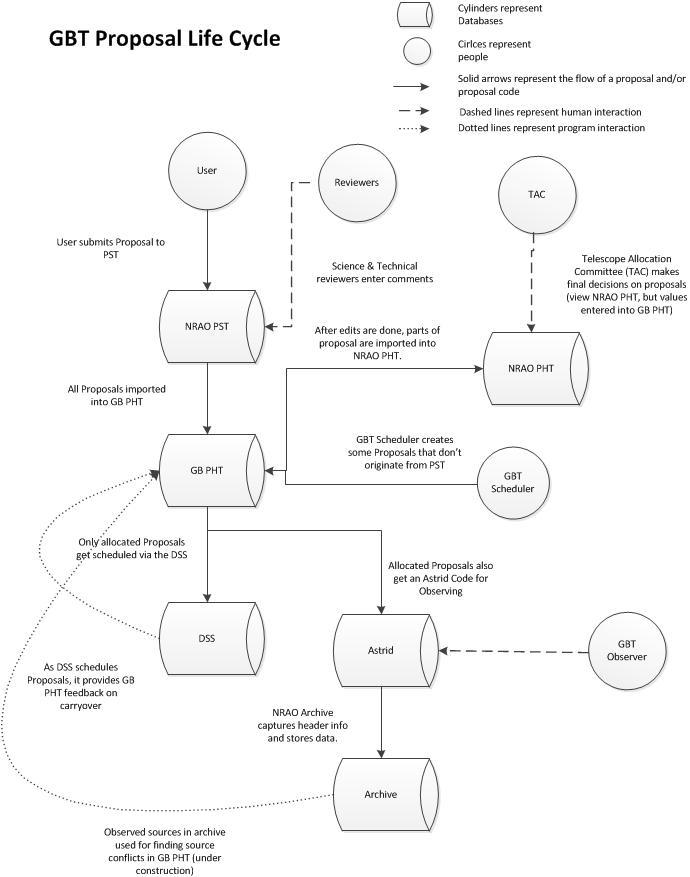
\includegraphics[width=0.8\textwidth]{ProposalLifeCycle.jpg}
\caption{GBT Proposal Life Cycle}
\label{proposal_life_cycle_image}
\end{figure}

Figure~\ref{proposal_life_cycle_image} shows the path(s) a GBT Proposal may take.
Here is a brief description of elements of this life cycle.  Note that details
are explained in other sections.

\begin{itemize}
\item Scientist submits a Proposal into the NRAO Proposal Submission Tool
(PST) (Sec.~\ref{pst_sec}) before the submission deadline, which is the first day of the Current
Semester; thus this new Proposal may begin observing by Next Semester.  This
is the beginning of the Proposal's life cycle.
\item All new proposals for the Next Semester are imported into the GB PHT (Sec.~\ref{gb_pht_sec}).
\item Science Review Panels and Technical Reviewers enter comments for each
Proposal in the PST.
\item Comments from Reviewers are later imported into GB PHT.
\item GBT Scheduler may optionaly add new Proposals directly into the GB PHT
\item GBT Scheduler edits Proposal in GB PHT
\item In preparation for the TAC meeting syncing is enabled between GB PHT and NRAO PHT (Sec.~\ref{nrao_pht_sec})
\item TAC meeting is held (about the middle of the Current Semester); TAC
feedback entered into GB PHT; changes propogated into NRAO PHT.  How does this
tie back into PST?
\item GBT Proposals that have been allocated time are given a Dynamic
Scheduling System (DSS) (Sec.~\ref{dss_sec}) project so that they can be scheduled on the GBT, and
a corresponding Astrid Code (version of the Proposal code) so that then can
actually observe on the GBT (Sec.~\ref{astrid_sec}).
\item Once the Next Semester starts, Scientists start observing their
Proposals on the GBT:
Time Accounting in the DSS feedsback into the GB PHT so that then next TAC
knows how much 'carryover' still needs to be observed, and observations are
archived (Sec.~\ref{archive_sec}).
\item Once a Proposal has observed enough of it's time on the GBT, it is
labeled as closed.  This is the end of the Proposal's life cycle.

\end{itemize}

\clearpage

\section{Proposal Submission Tool}\label{pst_sec}

TBF: what needs to be said about the PST?  

\section{GB Proposal Handling Tool}\label{gb_pht_sec}

The GB PHT is where all submitted Proposals from the PHT end up.  If a
Proposal is going to be allocated time and observe on the GBT, that decision
is entered here.

TBF: go into a detailed timeline here?


\section{NRAO Proposal Handling Tool}\label{nrao_pht_sec}

TBF: what to say here?


\section{GBT Dynamic Scheduling System}\label{dss_sec}

The GBT DSS is used for scheduling observations on the GBT \cite{}.

\subsection{DSS Projects and Sessions}

Once a Proposal has been allocated time by the TAC, it is 'exported' into the
DSS.  That is to say, the PHT's Proposal is given an associated DSS Project.
This Project has corresponding session's to the sessions in the Proposal,
however ...

The Proposal Code is used, without modification, for the DSS Project Code.

\subsection{Feedback to GB PHT}

As a DSS Project's Sessions are scheduled on the GBT, scientists manage their observing via Astrid (Sec.~\ref{astrid_sec}).  Utilitzing notes from the Operators Logs, the complex time accounting for these observations are determined in the DSS \cite{}.  As the 'time remaining' for a given Project's Session decreases, the GBT Scheduler decides when and if the Project is 'complete', that is, when it should be done with its observations.

The DSS Project's 'time remaining' and 'complete' status are feedback
programatically to the GB PHT (contrary to Figure~\ref{proposal_life_cycle_image}, the GB PHT and DSS actually share the same database).  This is so that when the next cycle of new
proposals begins (the Next Semester becomes the Current Semester), any given
Proposal that has a corresponding DSS Project can be correctly taken into
account in the 'carryover'.  So, a DSS Project that is not 'complete' and
still has 'time remaining' will contribute to the 'carryover' of the LST
Pressures \cite{marganian12b}.

This feedback mechanism is further utilized through the use of the DSS
'lookahead simulations'.  Simulations form the core of the DSS Science
Algorithms.  A simulation can be run from the present day to the end of the
Current Semester, with reports detailing which sessions ended up completeing,
or how much 'time remaining' they may have.  These predictions can be leveraged by the GBT Scheduler by entering the results into the GB PHT Sessions' 'Next Semester' fields \cite{marganian12a}, thus ensuring a more accurate 'carryover' result for the LST Pressure plots presented to the TAC.

\section{Astrid}\label{astrid_sec}

Astrid is the tool used by scientists for managing their GBT observations.
When a GBT Proposal is allocated time by the TAC, it is given a corresponding
DSS Project (Sec.~\ref{dss_sec}) and Astrid Project Code. Unlike the DSS Project
Code, the GB Proposal Code is modified before it becomes an Astrid Project
Code:

TBF: rules for turning Proposal Code into Astrid Project Code.

The Astrid Project Code is used in two significant ways:

\begin{itemize}
\item Scheduling Blocks (SB) - Observers make their actual observations by
submitting Scheduling Blocks via Astrid.  These SB's are managed via a
database, where they are organized via the Astrid Project Code.
\item Observation Data - Each time an observation is made via Astrid, the
Astrid Project Code must be chosen, as well as a 'session number' (no relation
to GB PHT and DSS essions).  The concatenation of these two values forms the
GBT M\&C Project Code, which in turn determines the directory where the
observation data is written to.
\end{itemize}

\section{Archive}\label{archive_sec}

TBF: what to say here, especially concerning the project code?

\section{Proposal Code Summary}\label{pcode_summary_sec}

Here we give a brief summary of the uses of the proposal code from the birth
of the proposal, through to it's observations on the GBT.
\begin{itemize}
\item NRAO PST: Proposal Code originates
\item GB PHT: Proposal Code loses '\' character
\item DSS: Proposal Code reused without modification
\item Astrid: Proposal Code altered to become Astrid Project Code.
Concatenated with 'session number' to label data.
\item Archive: TBF?
\end{itemize}

\subsubsection{Proposal Code Example}

\begin{itemize}
\item Scientist submits proposal at 2012-07-31 11:59:59.  It is assigned
Proposal Code GBT/13A-014
\item Proposals for semester 13A are imported on 2012-08-01 (first day of semester 12B).  Proposal code is changed to GBT13A-014.
\item Proposal is allocated time by TAC on 2012-10-13.  Proposals is given an associated DSS Project with Project Code GBT13A-014, and a corresponding Astrid Project Code of AGBT13A\_014.
\item Scientist observes Project after 13A starts (2013-02-01).  Their first observing session is labeled '01', so their data is stored in 'AGBT13A\_014\_01'.
\item Archive: TBF?
\end{itemize}

\section{Exceptions}\label{exceptions_sec}

You can't have rules without exceptions.  Here's ours:  GBT Maintenance,
Shutdown and Testing.  These types of activities don't follow the same life
cycle path as 'astronomical' proposals.  These actually originate in the DSS,
and are later exported to the GB PHT.  They never are reviewed by the TAC, and
are treated differently when calculating LST Pressures \cite{marganian12b}.


\begin{thebibliography}{}
\bibitem[Marganian(2012)]{marganian12a}
  Marganian, Paul, 2012, ``PHT Time Accounting''
  PH/PN001.0
\bibitem[Marganian(2012)]{marganian12b}
  Marganian, Paul, 2012, ``PHT LST Pressures''
  PH/PN002.0
\bibitem[Marganian(2010)]{marganian10a}
  Marganian, Paul, 2010, ``DSS Time Accounting''
  DS/PN011.0
\end{thebibliography}{}

\end{document}




















